% The README's annotated screenshot (docs/assets/appshot.png). Build: Tools/readme/build.sh.
%
% app.png is one window capture WITH its native shadow (screencapture -l, no -o), so the rounded
% corners, the hairline and the shadow are the system's own and read on a white page. The context
% menu is a separate window that -l cannot capture: it comes from a screen-region capture taken in
% the same instant and is pasted over the menu's own rectangle only, seams checked pixel-exact.
%
% Coordinates are given in the window's 2000-wide display space (the size the window was viewed
% at while picking targets); \W maps them into app.png, where the window sits at (112,76) and is
% 2560x1280. Same callout style as the paper's appshot: black orthogonal polylines, a dot at both
% ends, labels outside the window in a band above and a band below.
\documentclass[border=4pt]{standalone}
\usepackage[T1]{fontenc}
\usepackage{newtxtext}
\usepackage{tikz}
\begin{document}
\begin{tikzpicture}[
  fname/.style={font=\scriptsize\bfseries, align=left, inner sep=1pt},
  fdesc/.style={font=\scriptsize, align=left, inner sep=1pt},
  ln/.style={draw=black, line width=0.5pt, rounded corners=1.5pt},
  dot/.style={circle, fill=black, inner sep=0pt, minimum size=2.4pt},
]
\node[anchor=north west, inner sep=0] (img) at (0,0) {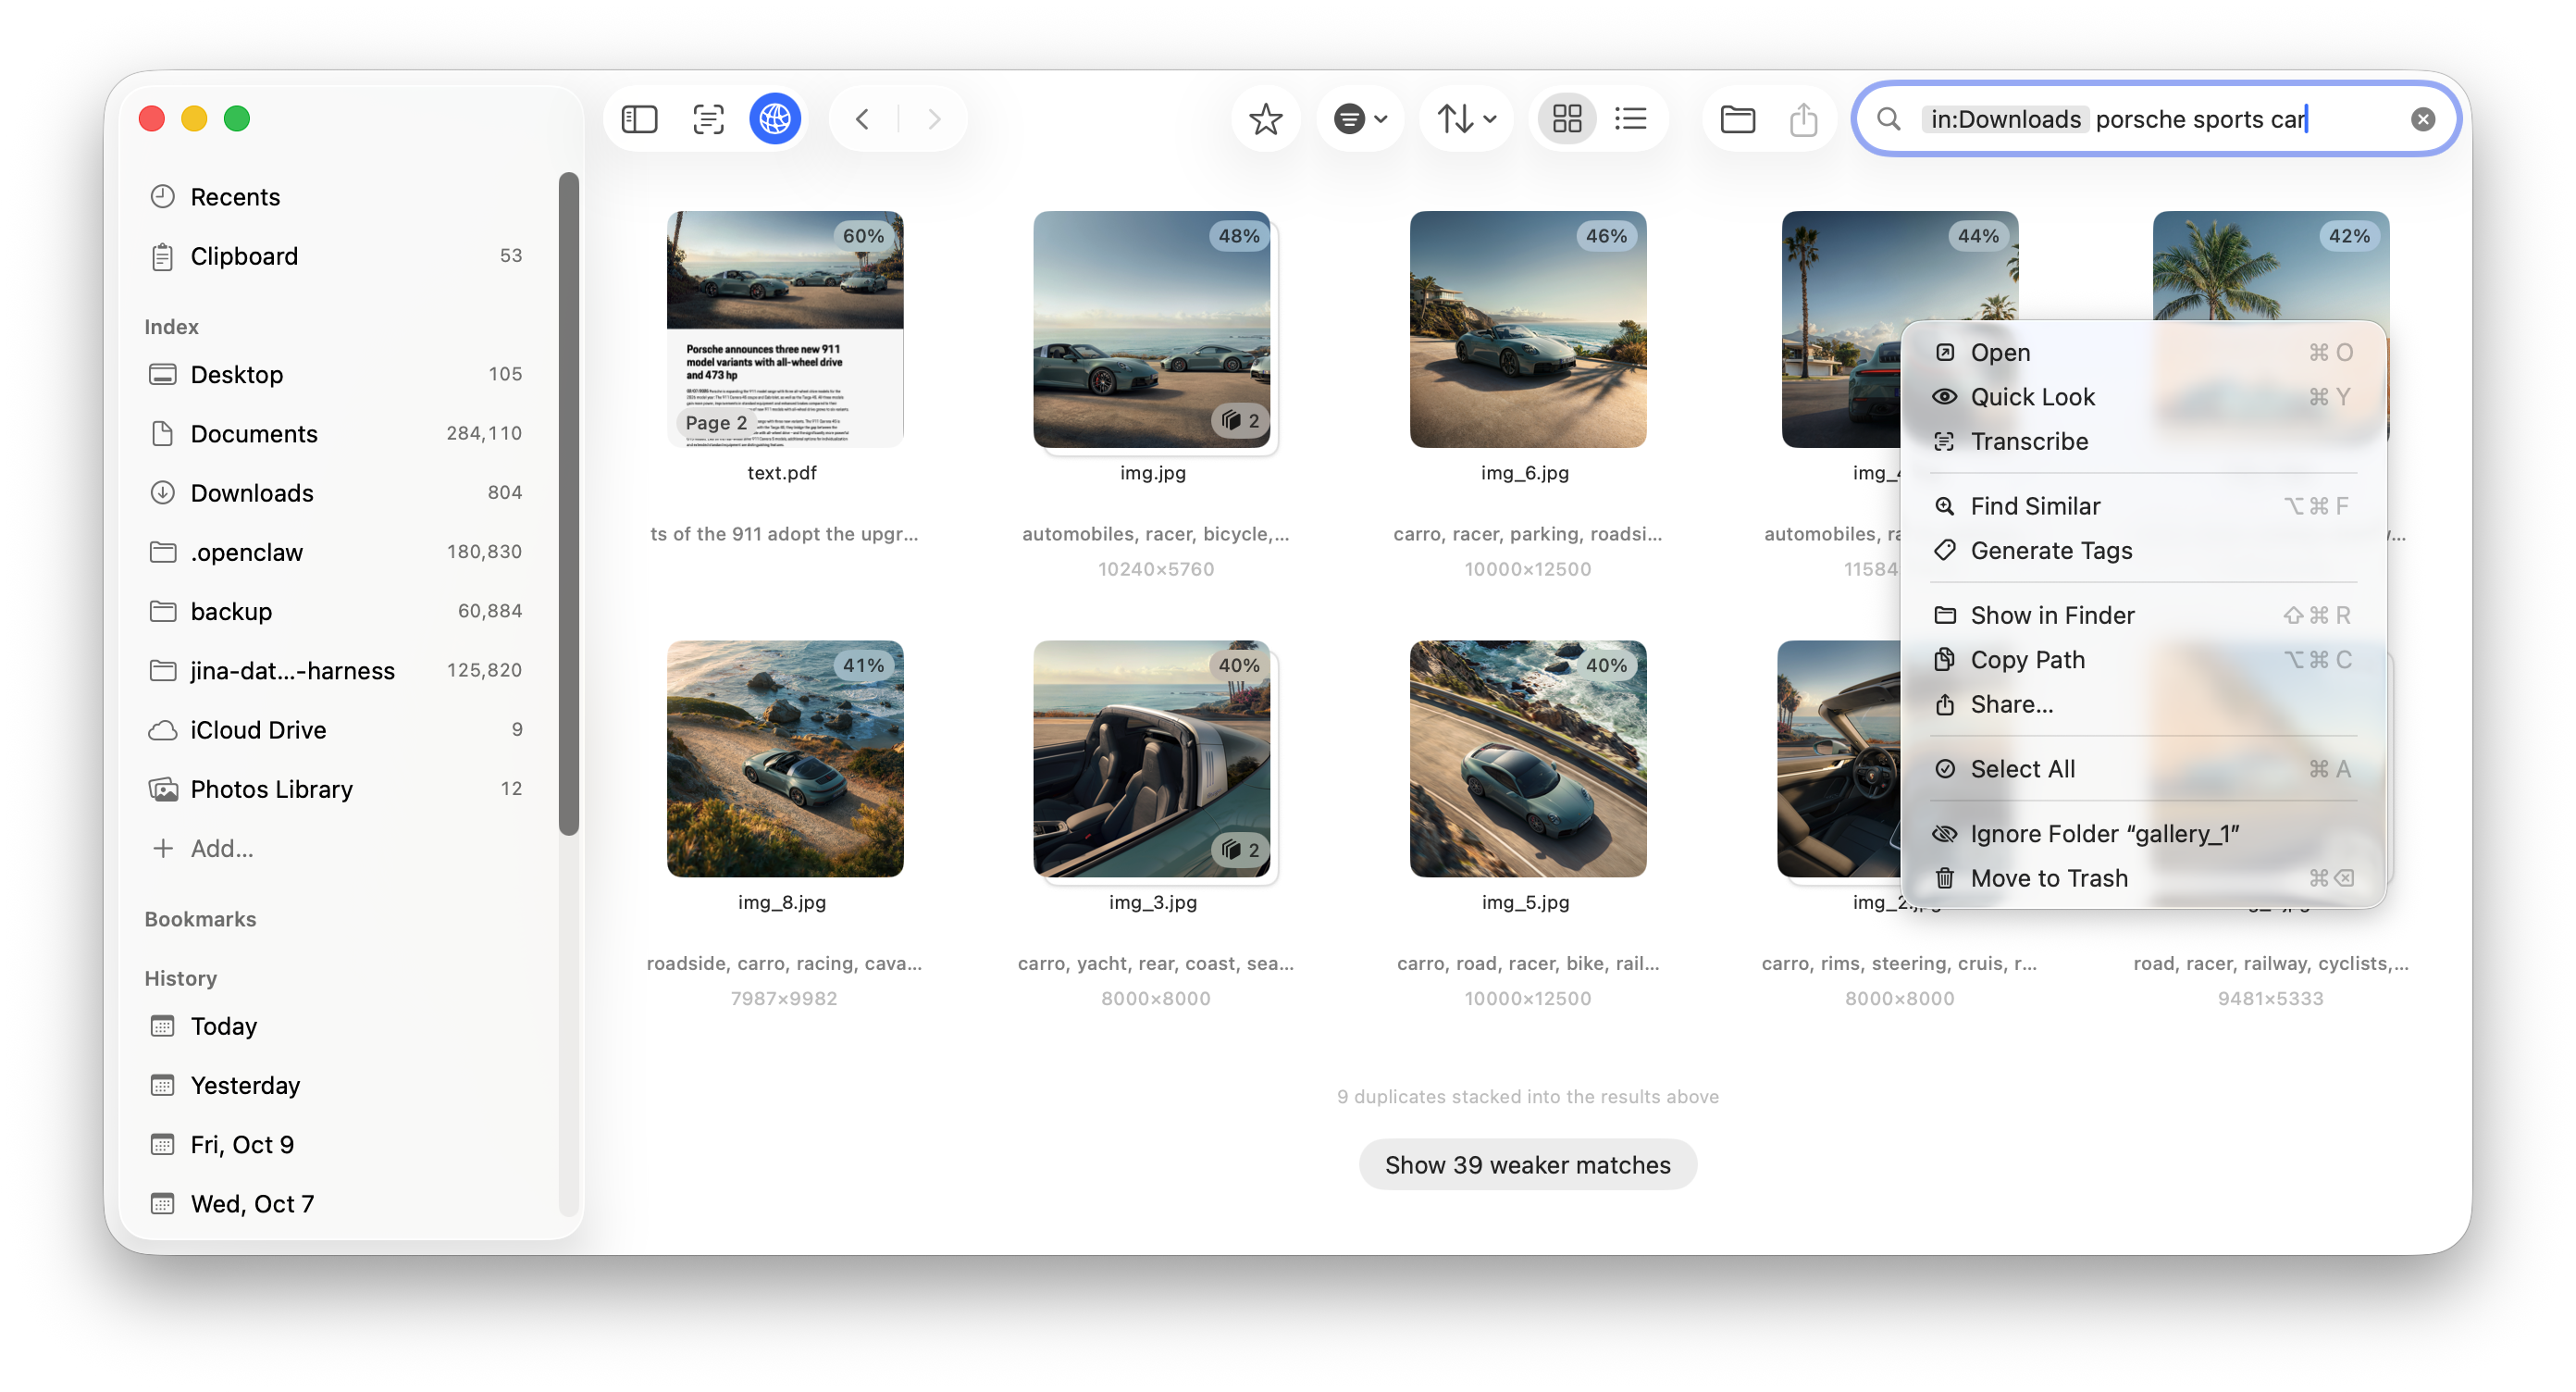
\includegraphics[width=18cm]{app.png}};
\begin{scope}[x=18cm/2784, y=-18cm/2784]
\def\X#1{{112+1.28*(#1)}}
\def\Y#1{{76+1.28*(#1)}}
% Band rows (app.png pixels, y down): name and description baselines, and where the leaders start.
\def\TN{-108} \def\TS{-60} \def\TD{-30}
\def\BN{1488} \def\BS{1536} \def\BD{1440}

% ---------------- top band ----------------
\node[fname, anchor=base west] at (\X{0},\TN) {Watched folders};
\node[fdesc, anchor=base west] at (\X{0},\TS) {indexed and kept current};
\draw[ln] (\X{234},\TD) -- (\X{234},\Y{307});
\node[dot] at (\X{234},\TD) {}; \node[dot] at (\X{234},\Y{307}) {};

\node[fname, anchor=base west] at (\X{400},\TN) {Page and line};
\node[fdesc, anchor=base west] at (\X{400},\TS) {where in the file it matched};
\draw[ln] (\X{539},\TD) -- (\X{539},\Y{297});
\node[dot] at (\X{539},\TD) {}; \node[dot] at (\X{539},\Y{297}) {};

\node[fname, anchor=base west] at (\X{880},\TN) {Copies stacked};
\node[fdesc, anchor=base west] at (\X{880},\TS) {one tile per file, not per copy};
\draw[ln] (\X{900},\TD) -- (\X{900},\Y{98}) -- (\X{958},\Y{98}) -- (\X{958},\Y{292});
\node[dot] at (\X{900},\TD) {}; \node[dot] at (\X{958},\Y{292}) {};

\node[fname, anchor=base east] at (\X{2000},\TN) {Search by meaning};
\node[fdesc, anchor=base east] at (\X{2000},\TS) {an \texttt{in:} chip scopes it to a folder};
\draw[ln] (\X{1605},\TD) -- (\X{1605},\Y{41});
\node[dot] at (\X{1605},\TD) {}; \node[dot] at (\X{1605},\Y{41}) {};

% ---------------- bottom band ----------------
\node[fname, anchor=base west] at (\X{0},\BN) {Search history};
\node[fdesc, anchor=base west] at (\X{0},\BS) {past queries, by day};
\draw[ln] (\X{234},\BD) -- (\X{234},\Y{857});
\node[dot] at (\X{234},\BD) {}; \node[dot] at (\X{234},\Y{857}) {};

\node[fname, anchor=base west] at (\X{420},\BN) {Relevance};
\node[fdesc, anchor=base west] at (\X{420},\BS) {cosine similarity to the query};
\draw[ln] (\X{725},\BD) -- (\X{725},\Y{502}) -- (\X{662},\Y{502});
\node[dot] at (\X{725},\BD) {}; \node[dot] at (\X{662},\Y{502}) {};

\node[fname, anchor=base west] at (\X{960},\BN) {Text finds photos};
\node[fdesc, anchor=base west] at (\X{960},\BS) {one space for every file type};
\draw[ln] (\X{1020},\BD) -- (\X{1020},\Y{600}) -- (\X{1150},\Y{600});
\node[dot] at (\X{1020},\BD) {}; \node[dot] at (\X{1150},\Y{600}) {};

\node[fname, anchor=base east] at (\X{2000},\BN) {Native file actions};
\node[fdesc, anchor=base east] at (\X{2000},\BS) {Quick Look, Find Similar, Transcribe};
\draw[ln] (\X{1670},\BD) -- (\X{1670},\Y{725}) -- (\X{1790},\Y{725}) -- (\X{1790},\Y{682});
\node[dot] at (\X{1670},\BD) {}; \node[dot] at (\X{1790},\Y{682}) {};
\end{scope}
\end{tikzpicture}
\end{document}
